\section{Architettura del prodotto}

\subsection{Descrizione generale}
In fase di progettazione è stato deciso di dividere il sistema \emph{HD Viz} in due parti distinte: una web app e un server che riesca a recuperare i dati da diversi tipi di database.

La web app è in grado di recuperare i dati a partire da file csv o di collegarsi al server e recuperare i dati dal database. Sarà possibile scegliere diversi tipi di visualizzazioni e diverse opzioni per creare la visualizzazione più utile per l'analisi dei dati.

La parte server gestisce le chiamate API. Il suo scopo è di fare da interfaccia tra il client e il database a cui esso vuole collegarsi. Essendo possibile collegarsi a diversi tipi di database il server è in grado di gestire e uniformare le risposte delle query sia per database SQL che non.

\subsection{Architettura web app}
    \subsubsection{Descrizione}
    Per sviluppare la web app è stato deciso di utilizzare il pattern architetturale MVVM. Le principali motivazioni dietro questa scelta sono: 
    \begin{itemize}
        \item la web app è stata realizzata tramite React e il pattern MVVM è sembrato abbastanza semplice da integrare;
        \item permette di utilizzare i modelli e gli Store in altri contesti senza doverli modificare;
        \item permette di disaccoppiare la parte di \emph{presentation logic} e \emph{business logic}.
    \end{itemize}
    
    Il passaggio dei dati dai Model alle varie View avviene tramite l'utilizzo degli Store (\emph{Model View}). Grazie al \emph{Context} di React nelle View è possibile eseguire un binding tra le proprietà dei componenti React e gli attributi esposti dagli Store, inoltre è possibile eseguire un binding tra le funzioni dei componenti React e i metodi esposti dagli Store.
    
    L'aggiornamento dei dati e le notifiche dei cambiamenti a questi dati avviene grazie all'uso di \emph{MobX}, una libreria per l'implementazione del pattern \emph{Observer} non disponibile nativamente in React.
    
    Per la selezione di una visualizzazione e le operazioni che devono essere eseguite viene utilizzato il pattern \emph{Template Method}.
    Quando un utente seleziona una visualizzazione:
    \begin{itemize}
        \item viene inizializzato il corretto modello di visualizzazione tramite l'oggetto di tipo VisualizationType contenuto all'interno del VisualizationManager.
        \item vengono visualizzate le opzioni relative alla giusta visualizzazione scelta.
    \end{itemize}
    
    \pagebreak
    
    \subsubsection{Diagramma dei package}
    Segue il diagramma dei package della web app.
    
    \begin{figure}[htbp]
        \centering
        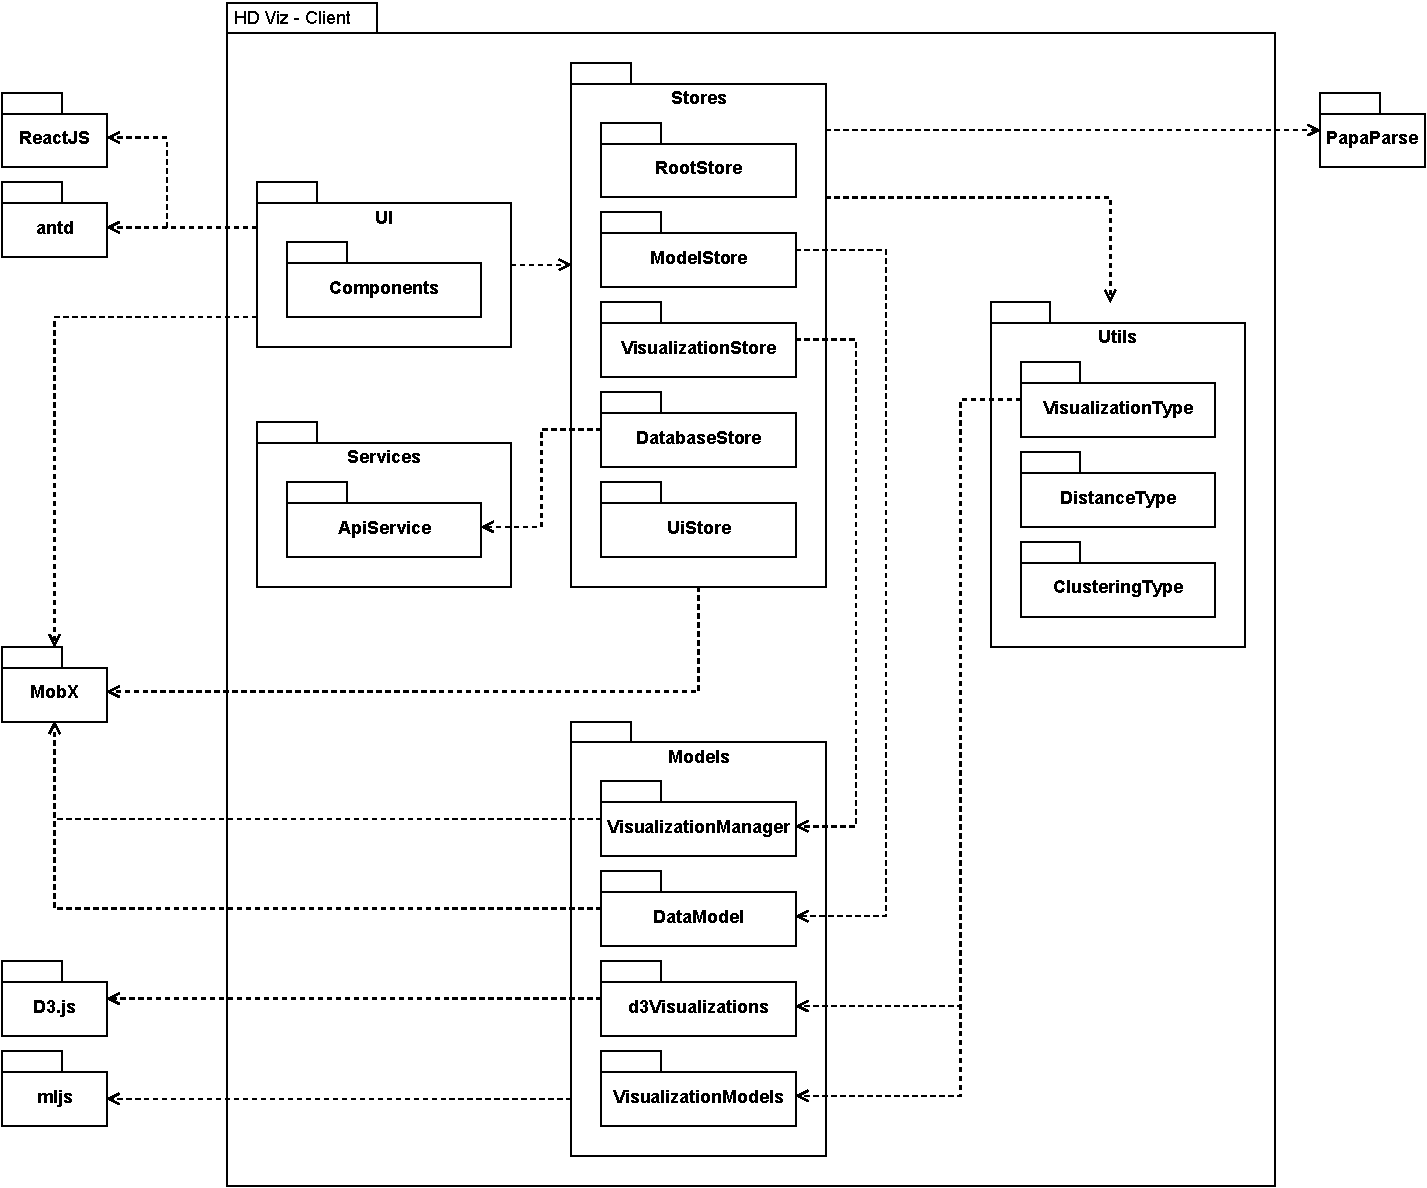
\includegraphics[width=1\textwidth]{source/img/package.pdf}
        \caption{Diagramma dei package della web app}
    \end{figure}
    
    \pagebreak
    
    \subsubsection{Diagrammi delle classi}
    Segue il diagramma delle classi della web app.
    \begin{figure}[H]
        \centering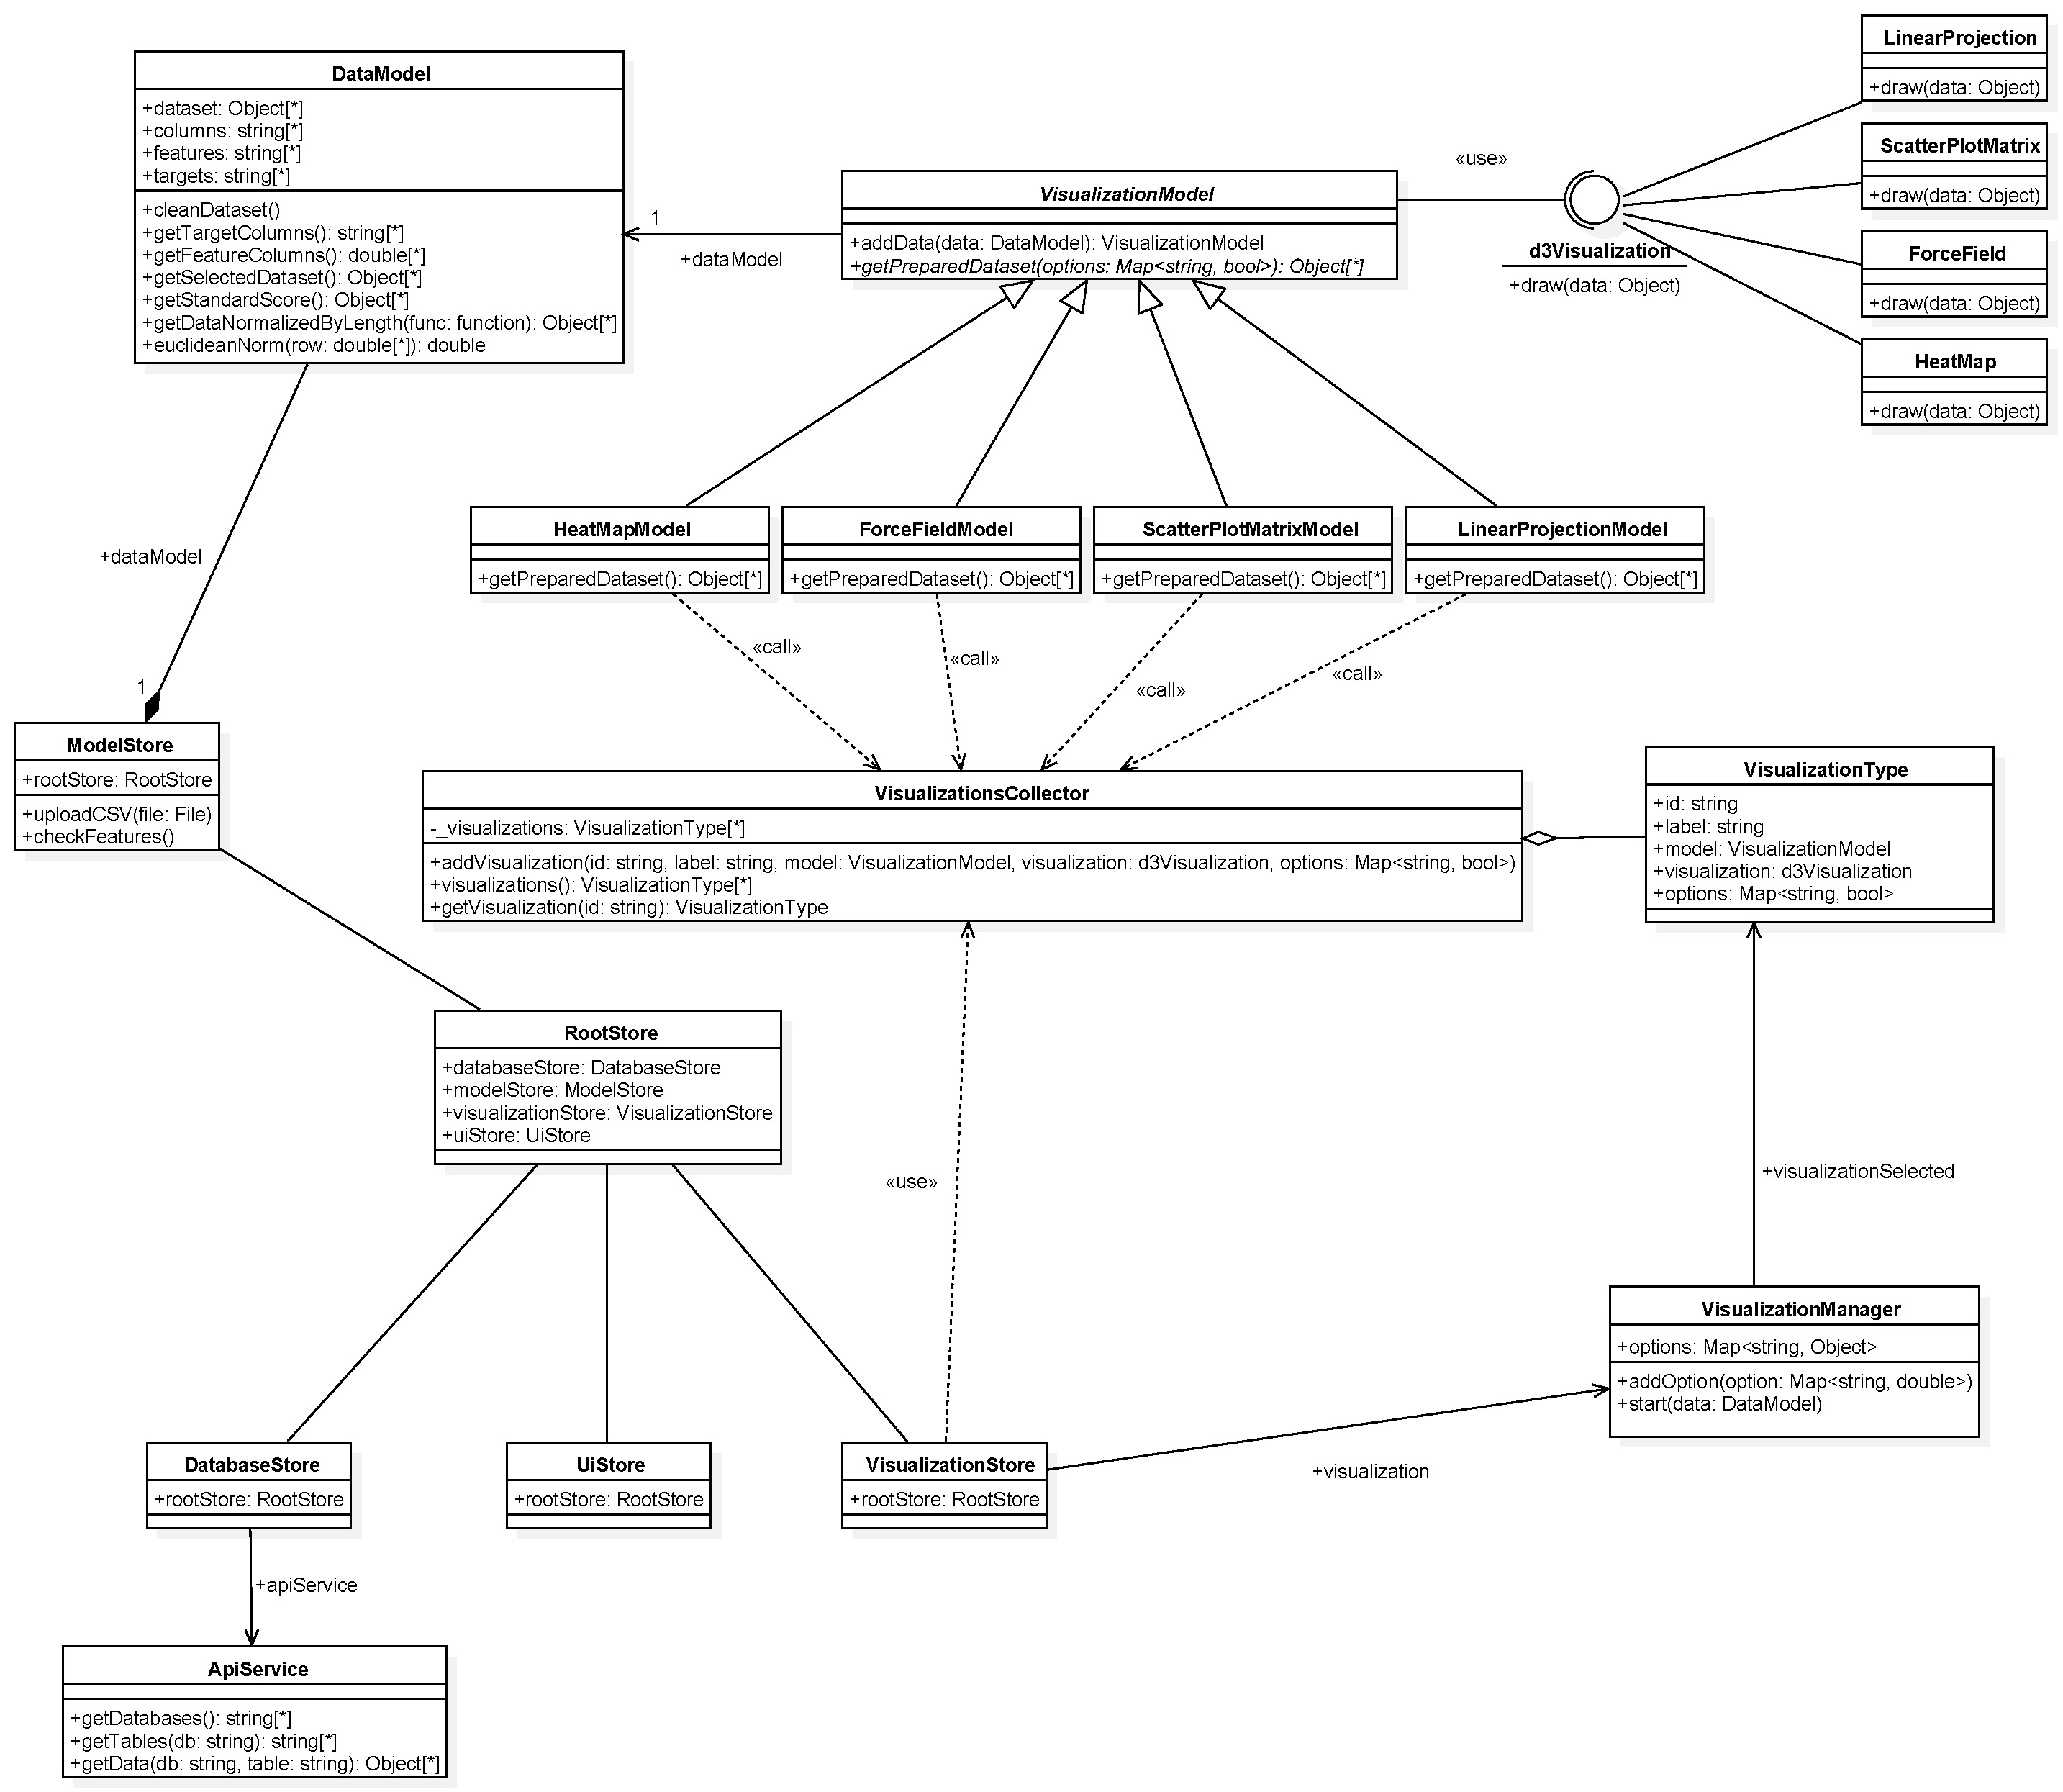
\includegraphics[width=1\textwidth]{source/img/classi.pdf}
        \caption{Diagramma delle classi della web app}
    \end{figure}
    
    \pagebreak
    
    \subsubsection{Diagrammi di sequenza}
        \paragraph{Diagramma di sequenza caricamento dati tramite CSV}
        Segue il diagramma di sequenza che modella le interazioni fra le classi coinvolte per il caricamento dei dati da file CSV.
            \begin{figure}[H]
                \centering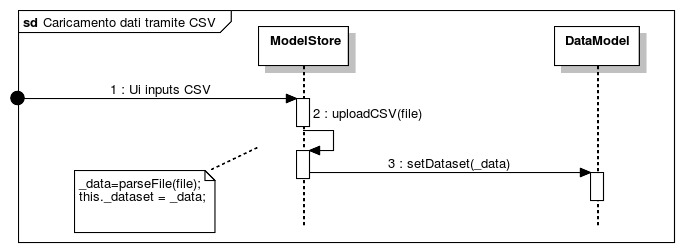
\includegraphics[width=1\textwidth]{source/img/sequenza1.jpeg}
                \caption{Diagramma di sequenza per il caricamento dati da file CSV}
            \end{figure}
            
        \paragraph{Diagramma di sequenza per la scelta del tipo di visualizzazione}
        Segue il diagramma di sequenza che modella le interazioni fra le classi coinvolte per la scelta del tipo di visualizzazione.
        \begin{figure}[H]
                \centering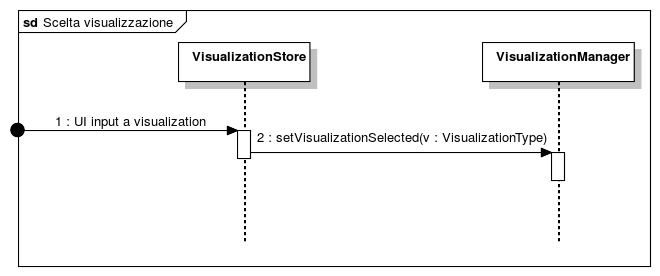
\includegraphics[width=1\textwidth]{source/img/sequenza2.jpeg}
                \caption{Diagramma di sequenza per la scelta del tipo di visualizzazione}
            \end{figure}
        \paragraph{Diagramma di sequenza per la selezione delle feature e target}
        Segue il diagramma di sequenza che modella le interazioni fra le classi coinvolte nella selezione delle feature e target.
        \begin{figure}[H]
                \centering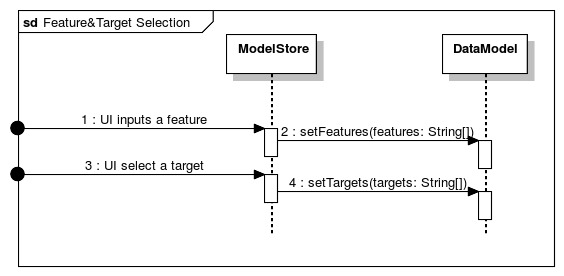
\includegraphics[width=1\textwidth]{source/img/sequenza3.jpeg}
                \caption{Diagramma di sequenza per la selezione delle feature e target}
            \end{figure}
        
        \paragraph{Diagramma di sequenza per la selezione della distanza (opzioni generiche)}
        Segue il diagramma di sequenza che modella le interazioni fra le classi coinvolte per la selezione della distanza(e in generale di tutte le opzioni riguardanti la manipolazione del dataset).
        \begin{figure}[H]
                \centering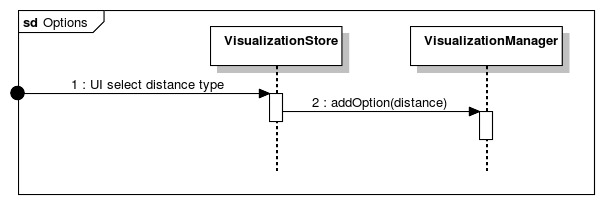
\includegraphics[width=1\textwidth]{source/img/sequenza4.jpeg}
                \caption{Diagramma di sequenza per la selezione del tipo di distanza da utilizzare per la matrice}
        \end{figure}
        
        \paragraph{Diagramma di sequenza per la visualizzazione del grafico selezionato}
        Segue il diagramma di sequenza che modella le interazioni fra le classi coinvolte per la visualizzazione del grafico scelto.
        \begin{figure}[H]
                \centering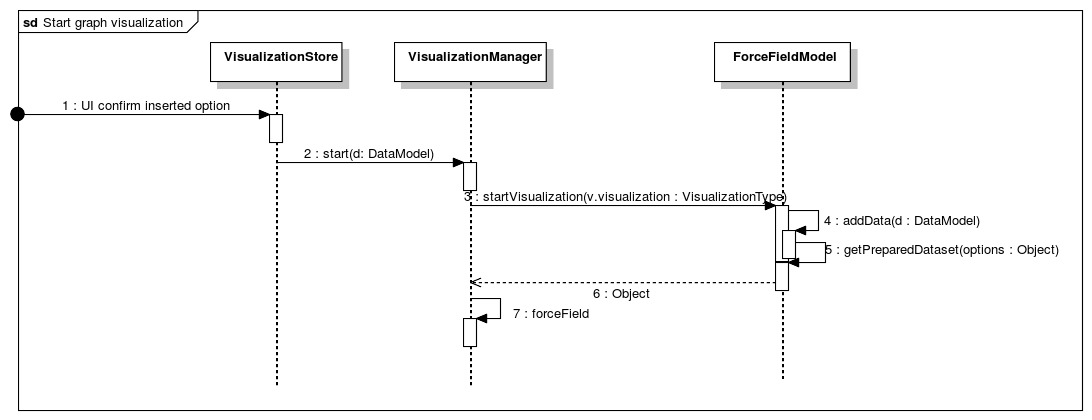
\includegraphics[width=1\textwidth]{source/img/sequenza5.jpeg}
                \caption{Diagramma di sequenza per la visualizzazione del grafico}
            \end{figure}
        
        
    \subsubsection{Design Pattern utilizzati}
        Sono stati individuati due differenti pattern, entrambi utilizzati nel model:
        \begin{itemize}
            \item Template method;
            \item Facade.
        \end{itemize}
        Per quanto riguarda il \textbf{Template method pattern}: la classe VisualizationModel è il template e i diversi tipi di visualizzazioni (ForceFieldModel, HeatMapModel,...) devono implementare VisualizationModel e in particolare il metodo \texttt{getPreparedDataset()}. La realizzazione di tale pattern, per le caratteristiche di JavaScript, richiede di inserire all'interno dei metodi astratti un'eccezione, in questo modo le varie generalizzazioni sono obbligate a implementarli. L'utilizzo di questo pattern ha permesso di evitare un'espressione switch per richiamare la visualizzazione richiesta e facilita l'estensione di \emph{HD viz}.
        
        Allo scopo di semplificare le interazioni con il modello è stata creata una classe VisualizationManager, che funge da \textbf{Facade}. VisualizationManager fornisce una interfaccia semplificata alle componenti Store.
        
        \pagebreak
        
\subsection{Architettura server}
    \subsubsection{Descrizione}
    L'architettura server è composta da 5 moduli:
    \begin{itemize}
            \item index.js è il primo modulo eseguito e gestisce le richieste e le risposte dell'API.
            \item  controller.js ha come scopo l'indirizzamento del codice in base al tipo di database al quale ci si vuole connettere.
            \item SQL-Function.js il quale contiene le funzioni eseguite dai database di tipo SQL.
            \item Connection.js gestisce le diverse connessioni ai database.
            \item NoSQL-Function.js che contiene le funzioni per i database NoSQL.
        \end{itemize}
    Avendo la necessità di gestire connessioni a database SQL e non, abbiamo modularizzato il nostro server in modo tale da facilitare la manutenibiltà e la possibilità di integrare nuove funzionalità.
    
    La gestione delle richieste API è stata possibile tramite Express. Express è un framework per applicazioni web NodeJS che fornisce molti metodi di utilità HTTP che facilita la creazione di un API.
    
    \subsubsection{Diagrammi di sequenza}
    
    \paragraph{Diagramma di sequenza per la ricerca dei nomi dei database}
     Segue il diagramma di sequenza della chiamata API getDatabases che fornisce in risposta tutti i database al quale è possibile connettersi.
            \begin{figure}[H]
                \centering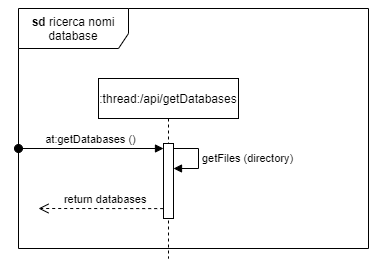
\includegraphics[width=0.6\textwidth]{source/img/API_getDatabases.png}
                \caption{Diagramma di sequenza per l'API getDatabases}
            \end{figure}
            \pagebreak;
            
    \paragraph{Diagramma di sequenza per la ricerca dei nomi delle tabelle del database}
        Segue il diagramma di sequenza della chiamata API getTable che fornisce in risposta i metadati delle tabelle presenti ne database richiesto.
            \begin{figure}[H]
                \centering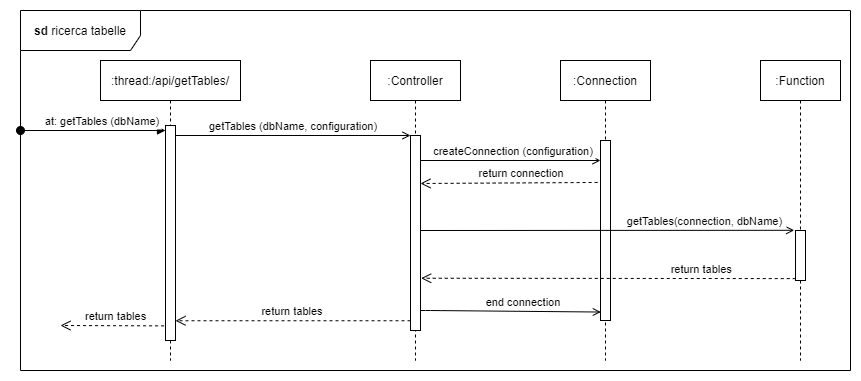
\includegraphics[width=1\textwidth]{source/img/API_getTable.png}
                \caption{Diagramma di sequenza per l'API getTable}
            \end{figure}
            
    \paragraph{Diagramma di sequenza per l'ottenimento dei dati della tabella selezionata}
    Segue il diagramma di sequenza della chiamata API getData che fornisce in risposta i metadati e dati della tabella selezionata.
            \begin{figure}[H]
                \centering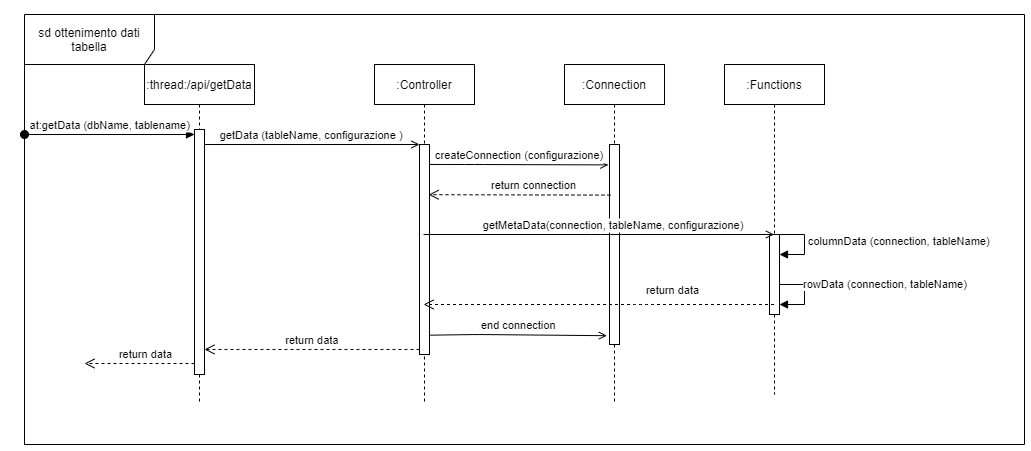
\includegraphics[width=1\textwidth]{source/img/API_getData.png}
                \caption{Diagramma di sequenza per l'API getData}
            \end{figure}